\documentclass[aspectratio=169,12pt]{beamer}
\usepackage{amsmath}
\usepackage{amssymb}
\usepackage[most]{tcolorbox}
\usepackage{tikz}
\usepackage{graphicx}
\usepackage[sfdefault,lf]{FiraSans}
\renewcommand{\familydefault}{\sfdefault}
\setlength{\parindent}{0pt}
\everymath{\displaystyle}

\setbeamertemplate{navigation symbols}{}
\setbeamertemplate{footline}{}
\setbeamertemplate{headline}{}

\definecolor{mmpageWhite}{HTML}{FCFBF7}
\definecolor{mmtanSoft}{HTML}{F7F5EF}
\definecolor{mmgreenDeep}{HTML}{244B2C}
\definecolor{mmgreenLeaf}{HTML}{5D8A56}
\definecolor{mmgreenSoft}{HTML}{E4EFD9}
\definecolor{mmtext}{HTML}{163221}

\setbeamercolor{background canvas}{bg=mmpageWhite}
\setbeamercolor{normal text}{fg=mmtext,bg=mmpageWhite}

\newtcolorbox{MMProblemCard}[1][]{enhanced,breakable=false,colback=white,colframe=black,boxrule=1.0pt,arc=5pt,left=3pt,right=3pt,top=2pt,bottom=2pt,before skip=0pt,after skip=0pt,height=0.26\textheight,valign=top,#1}
\newcommand{\KoruIcon}{\raisebox{-0.2em}{
\includegraphics[height=1.05em]{../../SITE/header-logo.png}}}
\newcommand{\HoeIcon}{\raisebox{-0.2em}{
\includegraphics[height=1.05em]{../../SITE/hoe.png}}}
\newcommand{\ScaffoldIcons}[1]{\ifcase#1\or \HoeIcon\or \HoeIcon\hspace{0.22em}\KoruIcon\or \KoruIcon\hspace{0.22em}\KoruIcon\hspace{0.22em}\KoruIcon\fi}
\newcommand{\WorksheetTitle}[2]{%
  {\colorbox{mmtanSoft}{\parbox[c][2.0em][c]{0.975\linewidth}{%
    \hspace{0.25em}{\Large\bfseries\textcolor{mmgreenDeep}{#1}\hfill\ScaffoldIcons{#2}}}}
  \par\vspace{0.08em}{\color{mmgreenLeaf}\rule{\linewidth}{2.0pt}}\par\vspace{0.04em}}
}
\newcommand{\MMProblem}[2]{\begin{MMProblemCard}\raggedright\small\textbf{#1.} #2\par\end{MMProblemCard}}

\setbeamertemplate{background}{
 \begin{tikzpicture}[remember picture,overlay]
 \draw[black,line width=1.5pt,rounded corners=10pt]
 ([xshift=0.45cm,yshift=-0.45cm]current page.north west)
 rectangle
 ([xshift=-0.45cm,yshift=0.45cm]current page.south east);
 \end{tikzpicture}
}

% Default worksheet generation rules:
% use notes-style beamer pages
% use bordered cards for individual problems
% target 9 problems per frame in a 3x3 grid
% target 3 frames per scaffold by default where content allows

\begin{document}\begin{frame}[t]
\WorksheetTitle{Push Tasks}
\vspace{-0.18em}
\begin{columns}[T,onlytextwidth]
\begin{column}{0.32\textwidth}\MMProblem{1}{Find the area.\\[0.4em]
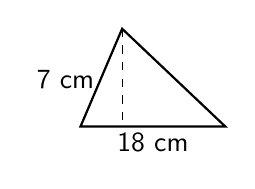
\begin{tikzpicture}[x=0.23cm,y=0.23cm,baseline=(current bounding box.center)]
  \coordinate (A) at (0,0);
  \coordinate (B) at (8,0);
  \coordinate (C) at (2.3,5.4);
  \draw[thick] (A)--(B)--(C)--cycle;
  \draw[dashed] (C)--(2.3,0);
  \node at (4,-0.9) {18 cm};
  \node at (1.3,2.6) [left] {7 cm};
\end{tikzpicture}}\end{column}
\begin{column}{0.32\textwidth}\MMProblem{2}{Find the area.\\[0.4em]
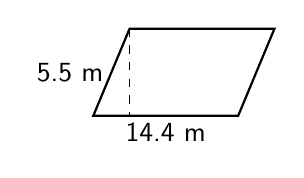
\begin{tikzpicture}[x=0.23cm,y=0.23cm,baseline=(current bounding box.center)]
  \coordinate (A) at (0,0);
  \coordinate (B) at (8,0);
  \coordinate (C) at (10,4.8);
  \coordinate (D) at (2,4.8);
  \draw[thick] (A)--(B)--(C)--(D)--cycle;
  \draw[dashed] (D)--(2,0);
  \node at (4,-0.9) {14.4 m};
  \node at (1.1,2.4) [left] {5.5 m};
\end{tikzpicture}}\end{column}
\begin{column}{0.32\textwidth}\MMProblem{3}{Find the area.\\[0.4em]
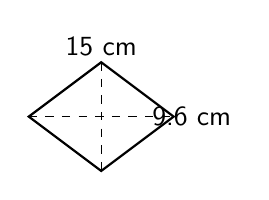
\begin{tikzpicture}[x=0.23cm,y=0.23cm,baseline=(current bounding box.center)]
  \coordinate (T) at (4,6);
  \coordinate (R) at (8,3);
  \coordinate (B) at (4,0);
  \coordinate (L) at (0,3);
  \draw[thick] (T)--(R)--(B)--(L)--cycle;
  \draw[dashed] (T)--(B);
  \draw[dashed] (L)--(R);
  \node at (4,6.9) {15 cm};
  \node at (9.0,3) {9.6 cm};
\end{tikzpicture}}\end{column}
\end{columns}
\vspace{0.45em}
\begin{columns}[T,onlytextwidth]
\begin{column}{0.32\textwidth}\MMProblem{4}{A rectangle has area 96 cm\mbox{$^2$} and length 12 cm. Find the width.}\end{column}
\begin{column}{0.32\textwidth}\MMProblem{5}{A square has area 196 m\mbox{$^2$}. Find its perimeter.}\end{column}
\begin{column}{0.32\textwidth}\MMProblem{6}{A triangle has area 45 cm\mbox{$^2$} and height 6 cm. Find the base.}\end{column}
\end{columns}
\vspace{0.45em}
\begin{columns}[T,onlytextwidth]
\begin{column}{0.32\textwidth}\MMProblem{7}{A parallelogram has the same base and height as a rectangle that is 11 cm by 4 cm. What is the area of the parallelogram?}\end{column}
\begin{column}{0.32\textwidth}\MMProblem{8}{A kite has area 84 cm\mbox{$^2$}. One diagonal is 14 cm. Find the other diagonal.}\end{column}
\begin{column}{0.32\textwidth}\MMProblem{9}{Which has greater area: a square of side 9 cm or a parallelogram with base 12 cm and height 7 cm? Show the difference.}\end{column}
\end{columns}
\end{frame}
\begin{frame}[t]
\WorksheetTitle{Push Tasks}
\vspace{-0.18em}
\begin{columns}[T,onlytextwidth]
\begin{column}{0.32\textwidth}\MMProblem{1}{A triangle and a kite both have area 54 cm\mbox{$^2$}. The triangle has base 12 cm. The kite has one diagonal 9 cm. Find the triangle's height and the kite's other diagonal.}\end{column}
\begin{column}{0.32\textwidth}\MMProblem{2}{A rectangle measures 18 cm by 7 cm. A triangle has the same area and base 14 cm. Find the triangle's height.}\end{column}
\begin{column}{0.32\textwidth}\MMProblem{3}{A student says, "A slanted side makes the area of a parallelogram bigger than a rectangle with the same base and perpendicular height." Explain why the student is wrong.}\end{column}
\end{columns}
\vspace{0.45em}
\begin{columns}[T,onlytextwidth]
\begin{column}{0.32\textwidth}\MMProblem{4}{A square and a triangle both have area 64 cm\mbox{$^2$}. The square has side 8 cm. If the triangle has base 16 cm, find its height.}\end{column}
\begin{column}{0.32\textwidth}\MMProblem{5}{A kite has diagonals 20 cm and 12 cm. A triangle has the same area and base 15 cm. Find the triangle's height.}\end{column}
\begin{column}{0.32\textwidth}\MMProblem{6}{The area of a parallelogram is 72 m\mbox{$^2$}. If the base is tripled and the perpendicular height is halved, what is the new area?}\end{column}
\end{columns}
\vspace{0.45em}
\begin{columns}[T,onlytextwidth]
\begin{column}{0.32\textwidth}\MMProblem{7}{Create two different rectangles with area 48 cm\mbox{$^2$} and explain how you know both are correct.}\end{column}
\begin{column}{0.32\textwidth}\MMProblem{8}{}\end{column}
\begin{column}{0.32\textwidth}\MMProblem{9}{}\end{column}
\end{columns}
\end{frame}
\end{document}
